\section{Neural Network}

The Convolutional Auto-Encoder is used to de-noise raw data from the CLAS12 drift chambers~\cite{Thomadakis:2022zcd}. 
The input and output for the network are matrices of size 36x112 representing hits in one sector of drift chambers. 
The training data was extracted from experimental data processed with CLAS12 reconstruction software. 
The raw hits (converted into a matrix) are used as an input for the neural network and a matrix constructed 
only from hits that belong to reconstructed tracks as an output (see Figure~\ref{conv:trackfinding}). 
In the training data set multiple track hits were allowed in the output matrix, shown on Figure~\ref{conv:trackfinding}.
The structure of neural network can be seen on Figure~\ref{network:cnn_encoder}, where the input and the output are images
of size 36x112. Convolutional and Max Pool layers are used for encoding the image into smaller latent space and then
decoding into an an output image (of same size as input) that contains only the desired pixels activated.

\begin{figure}[!h]
\begin{center}
 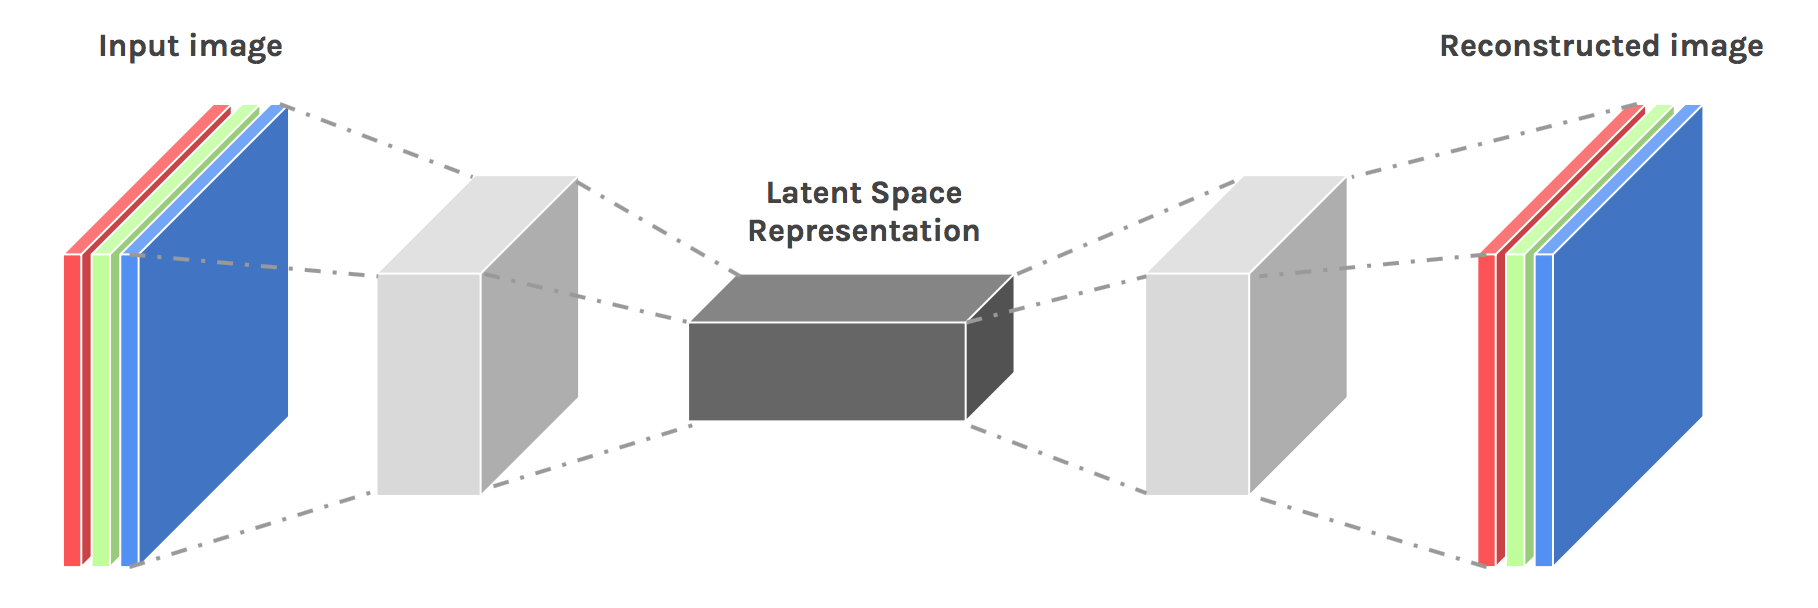
\includegraphics[width=5.1in]{images/convolutional-autoencoder.png}
\caption {De-noising Convolutional Auto-Encoder architecture. }
 \label{network:cnn_encoder}
 \end{center}
\end{figure}

The networks are validated on experimental data where the number of hits along the 
track trajectory from de-noised are compared to the hits reconstructed by conventional algorithm
as part of a valid track. An example of comparison can be seen in Figure~\ref{network:cnn_results} 
where raw data (left column) are shown along with data with hits belonging to reconstructed tracks 
identified by the conventional tracking algorithm (middle column) and 
reduced data processed by de-noising neural network (right column).

\begin{figure}[!h]
\begin{center}
 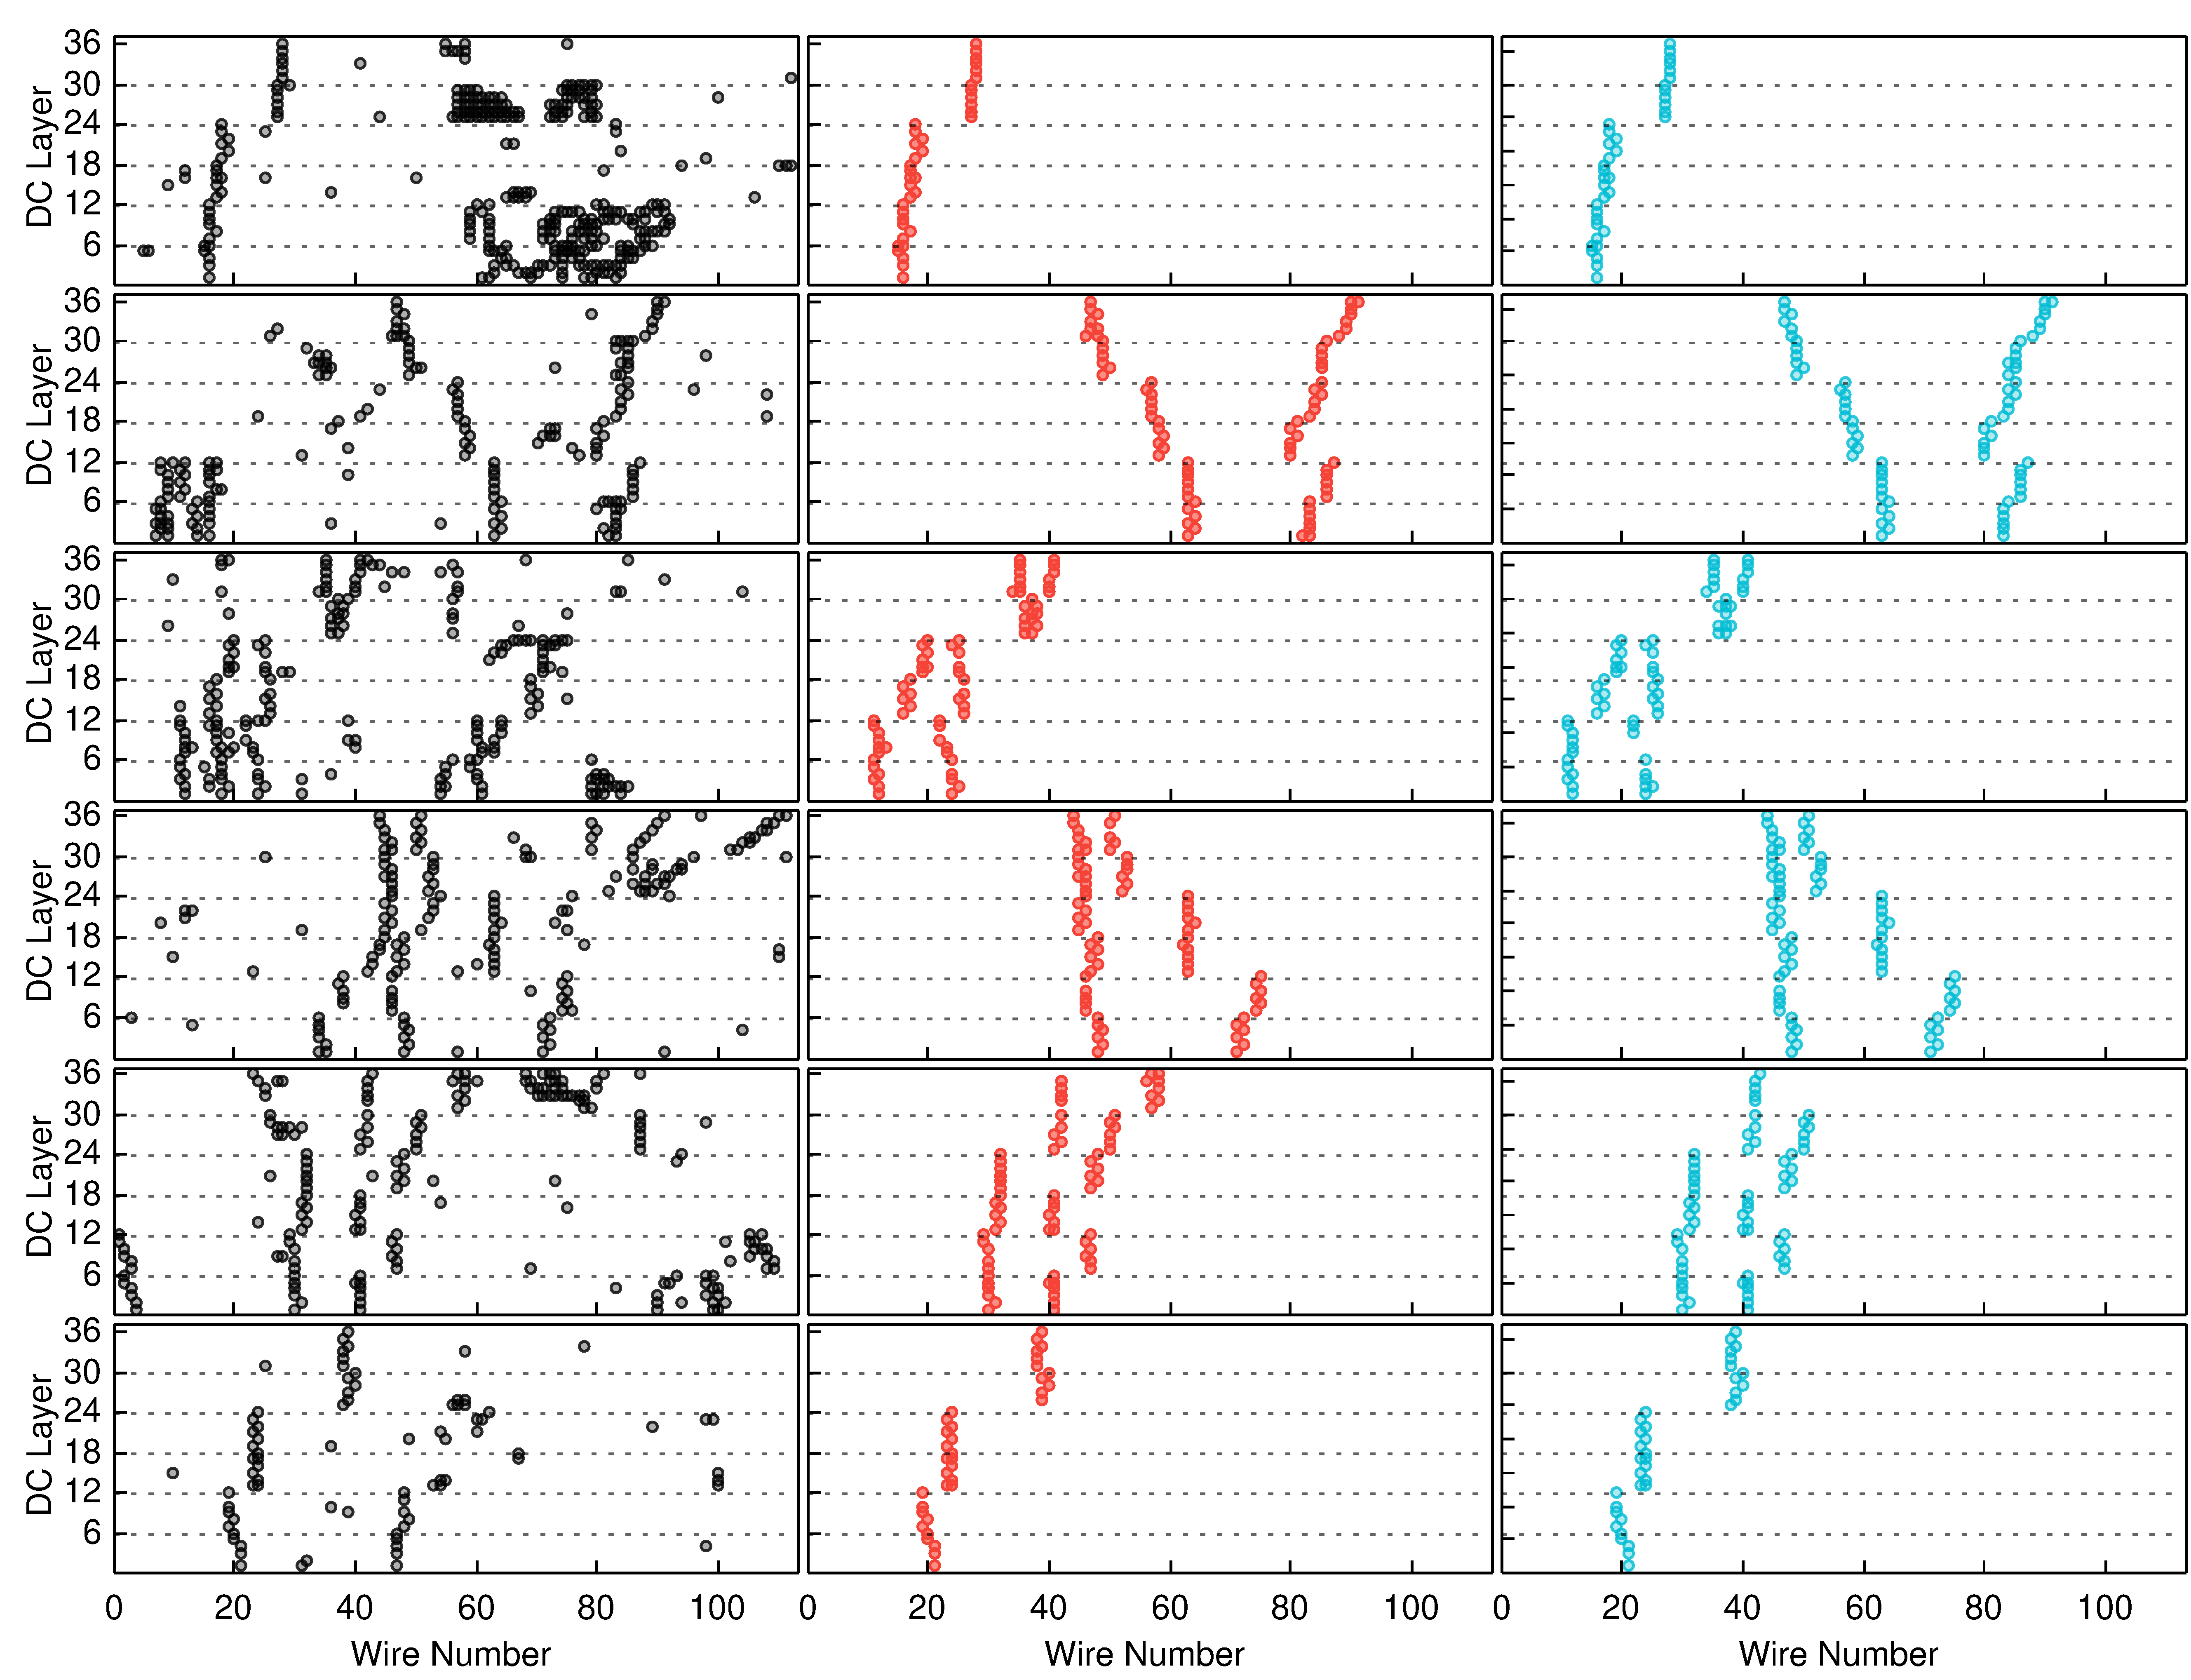
\includegraphics[width=5.8in]{images/cnn_denoise_results.pdf}
\caption {Results from the de-noising auto-encoder. The raw signal hits are shown
in the left column for 5 random events, along with hits reconstructed by the 
CLAS12 tracking algorithm in the middle column. The resulting  hits matrix 
from the de-noising raw hits are shown in the right column. (Systematic studies 
of de-noiser performance can be found here~\cite{Thomadakis:2022zcd})}
 \label{network:cnn_results}
 \end{center}
\end{figure}

As can be seen from the figure, the de-noising neural network removes all background hits not 
associated with a track, while preserving hits belonging to a track. 
Systematic studies~\cite{Thomadakis:2022zcd} showed that more than 
$95\%$ of the track related hits are preserved in the output of de-noiser while 
background hits are significantly suppressed for normal experimental conditions of 45nA
incident beam current. Systematic studies showed that in more than $85\%$ of cases all 
6 clusters belonging to the track are fully identified by the algorithm after de-noising, 
and in more than $97\%$ of the cases 5 clusters from the original track are recovered. The CLAS12 
track reconstruction algorithm can reconstruct tracks with 6 or 5 clusters along the 
track trajectory, which means that even if some clusters are lost due to de-noising 
procedure the track efficiency does not suffer significantly from this.

For our implementation of de-nosing software we used TensorFlow/Keras~\cite{keras-website} to train 
and evaluate the network. The resulting network parameters (weights) were saved 
in a HDF5 file. The de-noiser implementation for the CLAS12 reconstruction software is 
done using DeepLearning4J~\cite{dl4j-website} which supports model imports 
through HDF5 files. 
The data analysis and data visualization are done using the GROOT~\cite{groot-github} visualization 
package, developed for the CLAS12 software infrastructure (in Java) and is publicly available 
through github releases. GROOT is also included in Jas4pp\cite{Chekanov:2020bja}  
(data-analysis framework for physics and detector studies). The de-noising is not yet implemented 
as a part of the CLAS12 reconstruction workflow, and works as a standalone package to process raw data before 
they are analyzed with reconstruction software.
